\chapter{대칭성 깨짐, 골드스톤 보손, 게이지 불변성}

광자와 비슷한 입자가 어떻게 질량을 얻을 수 있는지 이해하고자 한다. 그것이 우리가 도달하려는 지점이지만, 합리적인 출발점은 아니다. 게이지 장에 질량항을 직접 넣으면 이론을 일관되게 만드는 바로 그 게이지 불변성이 깨지는 것처럼 보인다. 이 문제를 피할 길을 찾으려면 먼저 다음 두 가지 개념을 제대로 이해해야 한다.
\begin{enumerate}
  \item 자발적 대칭성 깨짐, 특히 연속 대칭의 자발적 깨짐;
  \item 대칭 연산이 시공간의 점마다 달라질 수 있는 게이지 불변성.
\end{enumerate}
어느 개념도 구호만으로 대신할 수는 없다. 먼저 자석을 통해 첫 번째 개념을 세우고, 이를 스칼라 장 이론으로 옮겨 질량이 없는 골드스톤 모드를 살펴보겠다. 그런 다음 같은 \(U(1)\) 대칭성을 국소적으로 만들고, 그 결과 벡터 퍼텐셜과 공변 미분을 도입해야 한다는 점을 알아보겠다. 두 흐름은 마지막에야 나란히 놓을 것이다. 두 흐름이 실제로 결합하는 현상, 곧---힉스 현상---을 다음 강의에서 다룬다.

\section{대칭적인 법칙과 비대칭적인 바닥 상태}

\subsection{두 상태를 갖는 자석}

작은 자석들이 놓인 격자에서 시작하자. 각 스핀은 위나 아래를 향할 수 있고, 이웃한 스핀들은 같은 방향을 향할 때 에너지가 낮아진다. 3차원 정육면체 격자에서는 스핀마다 최근접 이웃이 여섯 개지만, 정확한 배위수는 중요하지 않다. 중요한 것은 다음 규칙이다.
\begin{equation}
  E_{\parallel}<E_{\rm antiparallel}.
\end{equation}
모든 스핀의 방향을 뒤집어도 미시적 규칙은 변하지 않는다.
\begin{equation}
  \uparrow\longleftrightarrow\downarrow.
\end{equation}
그런데도 최저 에너지 배치 각각은 대칭적이지 않다. 가능한 배치는 다음과 같다.
\begin{equation}
  \{\uparrow\uparrow\uparrow\cdots\},
  \qquad
  \{\downarrow\downarrow\downarrow\cdots\}.
\end{equation}
방정식은 두 배치를 모두 허용하지만, 온도가 낮은 거시적 시료는 둘 중 하나를 선택해야 한다.

이 선택은 놀라울 만큼 민감하다. 아주 멀리 떨어진 곳의 스핀 하나를 위쪽으로 고정하자. 그 이웃들은 그 스핀을 따라 정렬하려 하고, 다시 그 이웃들의 이웃들도 같은 방향을 선호하면서 정보가 시료 전체로 퍼져 나간다. 전체 계의 크기에 비하면 임의로 작을 수 있는 섭동이 바닥 상태 전체의 방향을 결정할 수 있다. 이것이 \emph{자발적} 대칭성 깨짐에서 말하는 불안정성이다.

\begin{classroomqa}
\audiencequestion{중성 입자도 자기장에서 방향이 정렬될 수 있나요?
\lecturetimestamp{00:05:14}}
\lecturerresponse{그렇습니다. 전기적으로 중성이라고 해서 자기 모멘트가 없는 것은 아닙니다. 중성자인 중성자는 내부의 하전 구성 요소 때문에 자기 모멘트를 갖습니다. 따라서 자기장은 중성자의 스핀 방향에 따라 차이를 만들 수 있습니다.}
\end{classroomqa}

\begin{classroomqa}
\audiencequestion{계의 방향 변화는 모든 곳에서 동시에 일어나나요? 방향을 바꾸는 파동이 여러 개 함께 존재할 수 있나요?
\lecturetimestamp{00:05:41--00:06:38}}
\lecturerresponse{변화는 전파됩니다. 한 영역이 이웃한 영역을 기울게 하며, 마치 3차원 도미노 배열처럼 교란이 파동으로 퍼져 나갑니다. 서로 다른 영역들이 독립적으로 방향을 선택하기 시작할 수 있으므로, 하나의 방향이 우세해지기 전까지 여러 전선과 여러 영역이 함께 존재할 수 있습니다. 대칭성이 연속 대칭이 되었을 때 바로 이런 파동을 다시 살펴보겠다.}
\end{classroomqa}

\subsection{명시적 대칭성 깨짐은 다른 이론이다}

이제 위쪽을 향하는 외부 자기장 속에 시료를 놓자. 고립된 스핀은 이미 위쪽을 향할 때 에너지가 더 낮다. 변환 \(\uparrow\leftrightarrow\downarrow\)을 해도 에너지가 더는 변하지 않는 것이 아니다. 선호하는 방향이 법칙 자체에 들어간 것이다. 이것이 \emph{명시적} 대칭성 깨짐이다.

시료가 어떻게 준비되었는지 몰라도 두 경우를 구별할 수 있다. 매우 큰 시료를 택해 왼쪽 경계는 위쪽으로, 오른쪽 경계는 아래쪽으로 고정하자. 벌크 자기장이 위쪽 방향을 명시적으로 선호한다면, 오른쪽 경계 조건의 영향은 짧은 거리까지만 미친다. 거시적인 아래쪽 영역을 유지하려면 부피에 비례하는 에너지를 치러야 하므로, 벌크가 에너지가 똑같이 낮은 두 상으로 나뉜 채 남아 있을 수 없다.

외부의 편향이 없으면 위쪽과 아래쪽 방향의 벌크 에너지는 같다. 이때 구속 조건 아래의 최저 에너지 상태는 위쪽 영역, 아래쪽 영역, 그리고 그 사이의 유한한 전이층으로 이루어진다. 경계면이 기하학적 중심에 놓일 필요는 없지만, 한 상이 다른 상을 지워 버리도록 만드는 부피 압력은 없다. 이 경계면은 \emph{영역 벽}이며, 이산 대칭성 깨짐에서 나타나는 대표적인 결함이다.

\begin{figure}[htbp]
\centering
\begin{adjustbox}{max width=\linewidth}
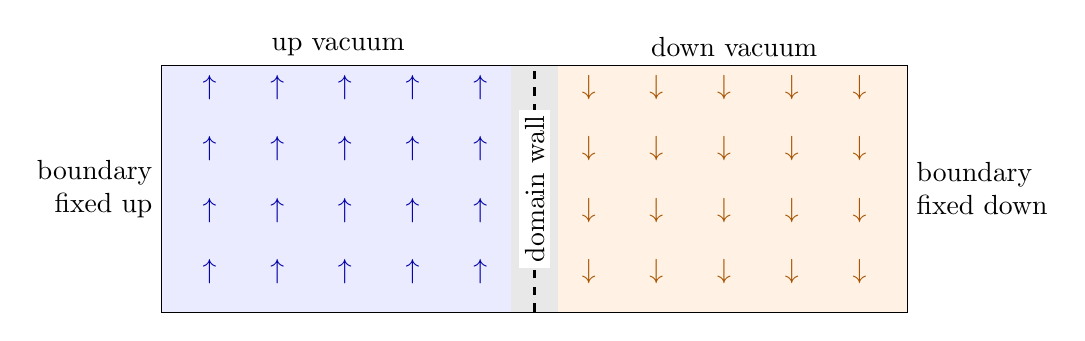
\begin{tikzpicture}[x=0.86cm,y=0.78cm]
  \draw[thick] (0,0) rectangle (11,4);
  \fill[blue!8] (0,0) rectangle (5.15,4);
  \fill[orange!10] (5.85,0) rectangle (11,4);
  \fill[gray!18] (5.15,0) rectangle (5.85,4);
  \foreach \x in {0.7,1.7,2.7,3.7,4.7}
    \foreach \y in {0.65,1.65,2.65,3.65}
      \node[blue!65!black] at (\x,\y) {$\uparrow$};
  \foreach \x in {6.3,7.3,8.3,9.3,10.3}
    \foreach \y in {0.65,1.65,2.65,3.65}
      \node[orange!65!black] at (\x,\y) {$\downarrow$};
  \draw[dashed,thick] (5.5,0) -- (5.5,4);
  \node[above] at (2.6,4) {up vacuum};
  \node[above] at (8.45,4) {down vacuum};
  \node[rotate=90,fill=white,inner sep=2pt] at (5.5,2) {domain wall};
  \node[left,align=right] at (0,2) {boundary\\fixed up};
  \node[right,align=left] at (11,2) {boundary\\fixed down};
\end{tikzpicture}
\end{adjustbox}
\caption{이산 대칭성의 자발적 깨짐을 확인하는 경계 조건 실험. 두 벌크 방향의 에너지가 같으므로 영역 벽이 거시적인 영역들을 가를 수 있다.}
\end{figure}

\begin{classroomqa}
\audiencequestion{최근접 이웃 사이의 상호작용만 있어야 이 논증이 성립하나요?
\lecturetimestamp{00:18:18}}
\lecturerresponse{아닙니다. 정렬을 선호하는 두 번째 이웃 상호작용이 있어도 세부 사항만 달라질 뿐 결론은 바뀌지 않습니다. 더 흥미로운 거동은 서로 다른 범위의 상호작용이 경쟁할 때 나타납니다--- 예컨대 최근접 이웃은 정렬을 선호하지만 차최근접 이웃은 반정렬을 선호하는 경우입니다. 그러면 좌절과 더 복잡한 질서상이 생기지만, 여기서 다루는 기본적인 구분은 달라지지 않습니다.}\end{classroomqa}

\begin{classroomqa}
\audiencequestion{\emph{자발적}이라는 말은 벽 내부의 큰 미분값을 가리키나요?
\lecturetimestamp{00:19:05}}
\lecturerresponse{아닙니다. 바탕이 되는 에너지에는 위쪽--아래쪽 선호가 없는데, 선택된 바닥 상태에는 그런 선호가 있다는 사실을 가리킵니다. 임의로 작은 섭동에도 극적으로 반응하는 것은 불안정성을 드러냅니다. 기울기는 경계면을 만드는 데 드는 비용만 알려 줍니다.}
\end{classroomqa}

\begin{classroomqa}
\audiencequestion{물질은 이미 두 상태 중 하나에 있었나요, 아니면 처음에는 어느 상태인지 알 수 없었나요?
\lecturetimestamp{00:19:40}}
\lecturerresponse{물질의 이력에 따라 다릅니다. 고온에서는 열운동 때문에 위쪽과 아래쪽 스핀이 섞여 자화의 평균값이 거의 0일 수 있습니다. 물질이 식으면서 여러 영역이 서로 다른 방향을 선택하고, 영역 벽이 생긴 뒤 영역들이 점차 커집니다. 어느 진공이 시료 대부분을 차지하게 될지는 우연과 미세한 환경 섭동에 달려 있습니다.}
\end{classroomqa}

\section{스칼라 장 이론으로 보는 같은 논증}

스핀을 실수 스칼라 장 \(\phi(\bm{x},t)\)으로 바꾸자. 계량과 정규화 관례를 하나로 정해 두고 다음과 같이 쓰자.
\begin{equation}
\begin{aligned}
  \mathcal L
  &=\frac12\,\partial_\mu\phi\,\partial^\mu\phi-V(\phi),
  \\
  \mathcal E
  &=\frac12\dot\phi^{\,2}+\frac12(\nabla\phi)^2+V(\phi).
\end{aligned}
  \label{eq:l07-real-scalar}
\end{equation}
\(\mathcal L\)의 상대론적 약기에는 양의 시간 미분 항과 음의 공간 기울기 항이 들어 있다. 해밀토니안 에너지 밀도에서는 두 항 모두 양의 기여를 한다.

서로 같은 두 최소점을 갖는 짝수 퍼텐셜을 택하자.
\begin{equation}
  V(\phi)=\frac{\lambda}{4}\left(\phi^2-f^2\right)^2,
  \qquad \lambda>0.
  \label{eq:l07-double-well}
\end{equation}
라그랑지안은 \(\phi\mapsto-\phi\)에 대해 불변이지만, 두 균일 진공 중 어느 하나가
\begin{equation}
  \phi(\bm{x})=+f,
  \qquad\hbox{or}\qquad
  \phi(\bm{x})=-f
\end{equation}
한쪽을 선택한다. 반면 \(\phi=0\)에 유일한 최소점을 갖는 퍼텐셜은 대칭적인 진공을 가지며 자발적으로 대칭성이 깨지지 않는다.

시료 한쪽에서는 \(\phi=+f\)을 고정하고 다른 쪽에서는 \(\phi=-f\)을 고정하자. 장은 비용 없이 갑자기 뛰어 바뀔 수 없다. 왜냐하면
\begin{equation}
  E_{\rm wall}
  =\int dx\left[
      \frac12\left(\frac{d\phi}{dx}\right)^2+V(\phi)-V(f)
    \right].
  \label{eq:l07-wall-energy}
\end{equation}
갑작스러운 변화는 \(d\phi/dx\)을 매우 크게 만든다. 따라서 에너지가 가장 낮은 영역 벽은 유한한 폭에 걸쳐 변화를 퍼뜨려, 기울기 에너지와 두 최소점 사이를 지날 때의 퍼텐셜 비용 사이에서 균형을 이룬다. 식~\eqref{eq:l07-double-well}의 퍼텐셜에 대한 익숙한 킨크 해는 다음과 같다.
\begin{equation}
  \phi_{\rm wall}(x)
  =f\tanh\!\left[f\sqrt{\frac{\lambda}{2}}\,(x-x_0)\right],
  \label{eq:l07-kink}
\end{equation}
이는 칠판에서 설명한 매끄러운 전이를 구체적으로 보여 준다.
\editorialnote{강의에서는 퍼텐셜의 형태와 기울기 항을 근거로 논증하지만 장 방정식 자체를 풀지는 않는다. 식 \eqref{eq:l07-kink}은 명시된 모형의 표준 해를 제시하여, 논증을 바꾸지 않으면서 정성적으로 논의한 영역 벽을 구체화한다.}

이중 우물을 조금 기울여 한 최소점이 더 낮아지게 하자. 그러면 라그랑지안 자체가 비대칭이 된다. 영역 벽이 일시적으로 나타날 수는 있지만, 에너지가 더 높은 거짓 진공이 벽에 압력을 가한다. 벽은 움직이고 에너지가 더 낮은 상이 커진다. 이는 외부 자기장에 의한 명시적 대칭성 깨짐에 해당하는 장 이론의 현상이다.

지금까지 다룬 대칭성은 이산적이었다. 입자물리학에서는 \(U(1)\), \(SU(2)\), \(SU(3)\) 같은 연속군이 중요하다. 연속 대칭에서는 결함의 양상이 달라지고 새로운 종류의 입자가 등장한다.

\section{복소장과 전역 \texorpdfstring{\(U(1)\)}{U(1)}}

\subsection{내부 평면에서의 회전}

다음과 같이 두자.
\begin{equation}
  \phi=\phi_R+i\phi_I,
  \qquad
  \phi^*=\phi_R-i\phi_I,
  \qquad
  \phi^*\phi=\phi_R^2+\phi_I^2.
  \label{eq:l07-components}
\end{equation}
\(\phi_R\)축과 \(\phi_I\)축은 내부 장 공간을 이루며, 보통 공간의 두 방향을 뜻하지 않는다. 복소 스칼라는 두 실수 스칼라 장을 묶어 내부 평면에서의 회전이 드러나게 한 것일 뿐이다.

\begin{figure}[htbp]
\centering
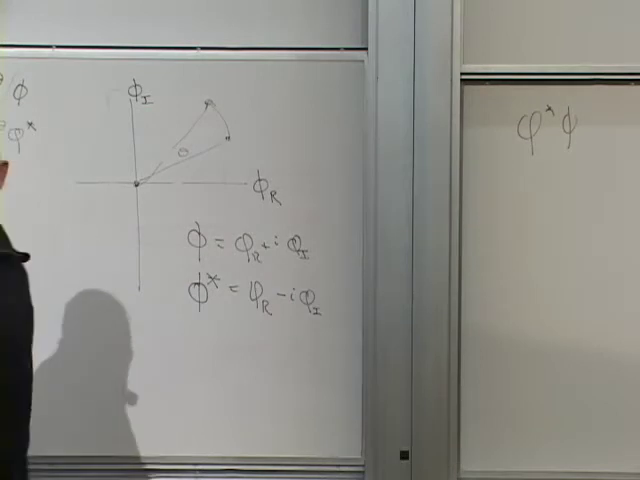
\includegraphics[width=0.80\textwidth]{lecture_07_figure_02.png}
\caption{\((\phi_R,\phi_I)\) 내부 평면 위의 복소장. 칠판에는 \(\phi\)과 \(\phi^*\)의 분해, 그리고 불변 반지름 \(\phi^*\phi\)이 기록되어 있다.}
\lectureframe{00:33:33}
\end{figure}

라그랑지안을 다음과 같이 두자.
\begin{equation}
  \mathcal L
  =\partial_\mu\phi^*\,\partial^\mu\phi
   -V(\phi^*\phi).
  \label{eq:l07-complex-lagrangian}
\end{equation}
복소장에는 관례적인 계수 \(1/2\)가 없다. 이 하나의 곱에 두 실수 성분의 운동항이 이미 모두 들어 있기 때문이다. 변환
\begin{equation}
  \phi'(x)=e^{i\theta}\phi(x),
  \qquad
  \phi^{*\prime}(x)=e^{-i\theta}\phi^*(x)
  \label{eq:l07-global-u1}
\end{equation}
은 모든 장의 값을 같은 각도만큼 회전시킨다. 여기서 \(\theta\)은 공간과 시간에 따라 변하지 않는 상수다. 프라임은 변환된 장을 나타내며, 미분을 뜻하지 않는다.

\(\theta\)이 상수이므로
\begin{equation}
  \partial_\mu\phi'=e^{i\theta}\partial_\mu\phi,
  \qquad
  \partial_\mu\phi^{*\prime}
  =e^{-i\theta}\partial_\mu\phi^*.
\end{equation}
위상 인자들이 운동항에서 서로 상쇄되고,
\(\phi^{*\prime}\phi'=\phi^*\phi\)도 성립한다. 따라서 \(\phi^*\phi\)에만 의존하는 퍼텐셜은 모두 같은 대칭성을 갖는다. \(\phi_R\)에만 의존하는 항은 내부 평면에서 한 방향을 택하게 하여 대칭성을 명시적으로 깨뜨린다.

\subsection{점 하나인 최소점과 원형 최소점}

대칭적인 퍼텐셜에는 정성적으로 다른 두 종류가 있다. 첫 번째는 원점에 유일한 최소점을 가지며, 예를 들면 다음과 같다.
\begin{equation}
  V_{\rm unbroken}=m^2\phi^*\phi,
  \qquad m^2>0.
\end{equation}
그래프는 회전 대칭인 포물면이다. 진공 \(\phi=0\)은 모든 회전에 대해 그대로이므로 대칭성이 깨지지 않는다.

이제 다음과 같이 택하자.
\begin{equation}
  V_{\rm broken}
  =-a\,\phi^*\phi+b(\phi^*\phi)^2,
  \qquad a,b>0.
  \label{eq:l07-mexican-hat}
\end{equation}
음의 이차항은 장을 원점에서 밀어내고, 양의 사차항은 장이 무한대로 발산하지 않게 한다. \(r^2=\phi^*\phi\)이라고 두고 최소화하면 다음을 얻는다.
\begin{equation}
  \frac{dV}{d(r^2)}=-a+2br^2=0,
  \qquad
  r^2=f^2=\frac{a}{2b}.
  \label{eq:l07-vacuum-radius}
\end{equation}
따라서 최소점들은 원을 이룬다. 퍼텐셜은 완벽한 회전 대칭을 유지하지만, 균일한 바닥 상태는 그 원 위의 한 점을 선택해야 한다.

\begin{figure}[htbp]
\centering
\includegraphics[width=0.72\textwidth]{lecture_07_figure_06.png}
\caption{회전면으로 그린 대칭성 깨짐 퍼텐셜. 원점은 불안정하고, 서로 축퇴된 최소점들은 원형 골짜기를 이룬다.}
\lectureframe{00:37:25}
\end{figure}

보통 공간의 각 점에 이 내부 평면의 작은 화살표 하나가 있다고 생각하자. 퍼텐셜은 화살표의 길이가 \(f\)이 되기를 요구한다. 기울기 에너지는 이웃한 화살표들이 거의 같은 방향을 향하도록 한다. 따라서 바닥 상태에서는 모든 곳의 각도가 같지만, 법칙은 어떤 각도도 선호하지 않는다. 이것이 연속 대칭성의 자발적 깨짐이다.

\section{영역 벽에서 매끄러운 비틀림으로}

경계 조건 실험을 다시 하자. 왼쪽 경계에서는 장을 진공점 \(A\)에 고정하고, 오른쪽 경계에서는 다른 진공점 \(B\)에 고정한다. 국소적으로 갑자기 뛰어 바뀌면 기울기가 커진다. 하지만 이산 대칭성의 경우와 달리, 장은 퍼텐셜의 최저점에 머문 채 원을 따라 연속적으로 변할 수 있다.

저에너지에서는 장을 \(\phi=f e^{i\alpha(x)}\)로 쓰자. 한 공간 차원에서 관련된 에너지는 다음과 같다.
\begin{equation}
  E[\alpha]
  =f^2\int_0^L dx\,\left(\frac{d\alpha}{dx}\right)^2.
  \label{eq:l07-angle-functional}
\end{equation}
양 끝의 각도를 고정하고 변분하면 다음을 얻는다.
\begin{equation}
  \frac{d^2\alpha}{dx^2}=0,
  \qquad
  \alpha(x)=\alpha_A+
    \frac{\alpha_B-\alpha_A}{L}\,x.
  \label{eq:l07-linear-twist}
\end{equation}
선호되는 배치는 시료 전체에 걸쳐 비틀림을 균일하게 퍼뜨린다. 그 에너지는 다음과 같이 스케일한다.
\begin{equation}
  E_{\rm twist}
  =f^2\frac{(\alpha_B-\alpha_A)^2}{L},
  \label{eq:l07-twist-energy}
\end{equation}
따라서 \(L\)을 늘리면 에너지를 임의로 작게 만들 수 있다.

\begin{figure}[htbp]
\centering
\begin{adjustbox}{max width=\linewidth}
\begin{tikzpicture}[x=0.95cm,y=0.95cm]
  \begin{scope}
    \draw[->] (0,0) -- (6.2,0) node[right] {$x$};
    \draw[->] (0,0) -- (0,3.5) node[above] {$\alpha(x)$};
    \draw[very thick,blue!70!black] (0.45,0.65) -- (5.7,2.85);
    \fill (0.45,0.65) circle (1.8pt) node[left] {$\alpha_A$};
    \fill (5.7,2.85) circle (1.8pt) node[right] {$\alpha_B$};
    \node at (3.1,-0.65) {physical space};
  \end{scope}
  \begin{scope}[xshift=9.2cm,yshift=1.65cm]
    \draw[thick] (0,0) circle (1.8);
    \fill (1.55,-0.92) circle (1.8pt) node[below right] {$A$};
    \fill (-0.45,1.74) circle (1.8pt) node[above] {$B$};
    \draw[very thick,blue!70!black,-{Latex[length=2.5mm]}]
      (1.55,-0.92) arc[start angle=-31,end angle=104,radius=1.8];
    \node at (0,-2.35) {vacuum circle};
  \end{scope}
\end{tikzpicture}
\end{adjustbox}
\caption{같은 저에너지 배치를 두 방식으로 나타냈다. 각도는 물리적 공간을 따라 선형적으로 변하고, 장은 내부 공간의 진공 원을 따라 짧은 호를 따른다.}
\end{figure}

\begin{classroomqa}
\audiencequestion{원을 따라가는 길이 두 가지일 수 있습니다. 장은 어느 길을 따르며, 더 긴 길에 갇힐 수도 있나요?
\lecturetimestamp{00:41:54}}
\lecturerresponse{일반적인 양 끝점에 대해서는 각도 변화가 더 짧은 경로가 기울기가 작으므로 에너지도 더 낮습니다. 서로 정반대인 양 끝점에서는 가장 간단한 두 경로의 에너지가 같습니다. 끝점 하나를 천천히 움직여 준비한 배치는 추가 감김수를 유지한 채 에너지 장벽 뒤에 갇힐 수 있습니다. 그러나 주어진 일반적인 양 끝점 쌍에 대해서는 비틀림이 없는 최단 경로가 바닥 상태입니다.}
\end{classroomqa}

\begin{classroomqa}
\audiencequestion{경로가 골짜기 바닥을 벗어나 내부를 가로질러 전체적으로 더 짧아질 수도 있나요?
\lecturetimestamp{00:43:32}}
\lecturerresponse{저에너지의 긴 시료에서는 반지름 방향 퍼텐셜을 올라가는 것이 유리하지 않다. 위의 변분법 계산에서 보았듯, 반지름을 진공값에 고정하고 각도를 선형적으로 변화시키는 것이 유효 에너지를 최소화한다. 특정 퍼텐셜을 가진 유한한 계에서는 반지름 방향 운동과 각도 운동을 함께 최소화할 수 있지만, 골드스톤 결론은 골짜기를 따라 부드럽게 움직이는 배치가 우세해지는 임의로 긴 파장의 극한에 관한 것이다.}
\end{classroomqa}

\begin{classroomqa}
\audiencequestion{원형 골짜기를 기울여 특정 각도를 더 낮게 만들면 무엇이 달라지나요?
\lecturetimestamp{00:44:33}}
\lecturerresponse{그러면 대칭성이 명시적으로 깨진다. 한 점이 참된 바닥 상태가 되고, 원을 따라 움직일 때 복원력이 생겨 각도 들뜸은 더 이상 정확히 질량이 없다.}
\end{classroomqa}

\section{영운동량 진동의 비용으로서의 질량}

매끄러운 비틀림은 에너지가 기울기에서만 비롯되는 장을 보여 준다. 이것이 왜 질량이 없는 입자를 뜻하는지 이해하려면 상대론적 분산 관계를 비교하자.
\begin{equation}
  \omega^2=\bm{k}^2+m^2.
  \label{eq:l07-dispersion}
\end{equation}
파동 \(e^{i(\bm{k}\cdot\bm{x}-\omega t)}\)은 운동량 \(\bm{k}\)을 갖는다. \(m=0\)이면 파장이 무한히 길어질수록 에너지는 0으로 다가간다.
\(\omega=|\bm{k}|\to0\). \(m\ne0\)이면 공간적으로 균일한 모드 \(\bm{k}=0\)도 각진동수 \(\omega=m\)로 계속 진동한다. 질량은 영운동량에서 남는 최소 에너지다.

이 구분은 라그랑지안에서도 드러난다. 항
\begin{equation}
  -\frac12m^2\varphi^2
\end{equation}
은 균일한 변위에도 복원력을 준다. 미분항만 있는 장에는 그런 복원력이 없다. 파장을 길게 만들수록 기울기 에너지는 0에 가까워진다.

\subsection{두 모드를 분리하는 극좌표}

대칭성이 깨진 복소장을 다음과 같이 쓰자.
\begin{equation}
  \phi(x)=\rho(x)e^{i\alpha(x)}.
  \label{eq:l07-polar}
\end{equation}
\(\rho\)와 \(\alpha\)은 모두 장이다. 미분하면 다음을 얻는다.
\begin{align}
  \partial_\mu\phi
  &=e^{i\alpha}
    \left(\partial_\mu\rho+i\rho\,\partial_\mu\alpha\right),\\
  \partial_\mu\phi^*
  &=e^{-i\alpha}
    \left(\partial_\mu\rho-i\rho\,\partial_\mu\alpha\right).
\end{align}
교차항이 상쇄되어 다음과 같이 남는다.
\begin{equation}
  \partial_\mu\phi^*\,\partial^\mu\phi
  =(\partial_\mu\rho)(\partial^\mu\rho)
   +\rho^2(\partial_\mu\alpha)(\partial^\mu\alpha).
  \label{eq:l07-polar-kinetic}
\end{equation}
\(\phi^*\phi=\rho^2\)이므로
\begin{equation}
  \mathcal L
  =(\partial\rho)^2+\rho^2(\partial\alpha)^2-V(\rho^2).
  \label{eq:l07-polar-lagrangian}
\end{equation}
퍼텐셜에는 \(\rho\)가 들어가지만 \(\alpha\)는 들어가지 않는다. 이 부재가 대칭성을 가장 유용한 형태로 보여 준다.

\begin{figure}[htbp]
\centering
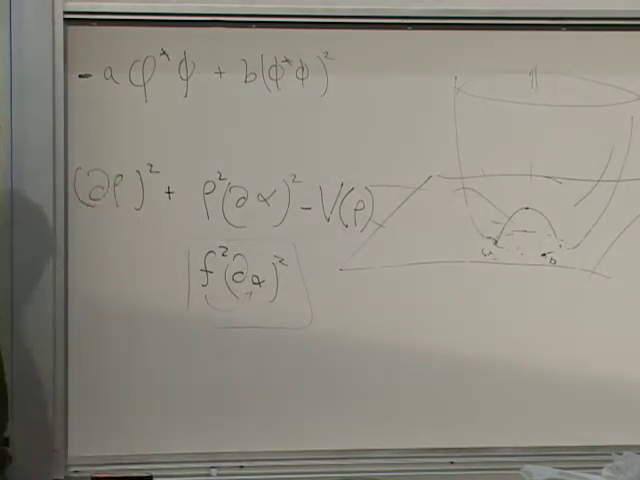
\includegraphics[width=0.88\textwidth]{lecture_07_figure_03.png}
\caption{극좌표 장의 라그랑지안, 상자로 표시한 저에너지 각도 항, 그리고 대칭성 깨짐 퍼텐셜. 반지름 방향 운동은 퍼텐셜을 거슬러 올라가고, 각도 방향 운동은 골짜기를 따른다.}
\lectureframe{00:56:40}
\end{figure}

매우 저에너지인 들뜸에서는 장이 \(\rho=f\)에 가깝게 유지된다. 그러면
\begin{equation}
  \mathcal L_{\rm angular}
  \simeq f^2(\partial_\mu\alpha)(\partial^\mu\alpha).
\end{equation}
계수 \(1/2\)에 관한 관례에 따라 정준 정규화된 각도 장을 다음과 같이 정의하자.
\begin{equation}
  \beta=\sqrt{2}\,f\alpha,
  \qquad
  \mathcal L_{\rm angular}
  =\frac12(\partial_\mu\beta)(\partial^\mu\beta).
  \label{eq:l07-goldstone-field}
\end{equation}
\(\beta^2\) 항은 없다. 이 각도 장의 양자는 질량이 없다. 이들이 골드스톤 보손이다.

반지름 방향 장의 거동은 다르다. \(\rho\)을 \(f\)에서 한꺼번에 변위시키면 골짜기로 되돌아가다가 지나쳐 진동한다. \(\rho=f+h\)이면 식~\eqref{eq:l07-mexican-hat}을 전개하여 다음을 얻는다.
\begin{equation}
  V(f+h)=V(f)+\frac12m_h^2h^2+\cdots,
\end{equation}
따라서 \(h\)에는 질량이 있다. 기하학적으로 각도 방향은 평평하고 반지름 방향은 굽어 있다.

\begin{classroomqa}
\audiencequestion{장이 방사 방향으로 변위되면 단순히 다시 아래로 떨어지는가? 그다음에는 무슨 일이 일어나는가?\lecturetimestamp{00:57:10}}
\lecturerresponse{각운동이 없으면 장은 최소점 쪽으로 떨어졌다가 그 지점을 지나쳐 방사 방향으로 진동한다. 공간적으로 균일한 진동은 공간 운동량이 없지만 주파수는 0이 아니며, 그 주파수가 방사 방향 여기의 질량이다. 이와 달리 공간적으로 균일한 각방향 변위는 다른 진공 상태에 도달하며, 복원력은 없다.}
\end{classroomqa}

이 예에서 골드스톤 원리의 내용은 다음과 같다. 연속 전역 대칭성이 자발적으로 깨지면 진공 다양체의 서로 독립적인 평탄 방향마다 질량이 없는 모드가 하나씩 생긴다.
\editorialnote{이 진술은 상대론적 장 이론의 통상적인 조건을 가정한다. 비상대론적 다체계에서는 난부--골드스톤 모드의 개수와 분산 관계가 더 미묘할 수 있지만, 이 상대론적 \(U(1)\) 모형에서는 강의의 장파장 결론이 여전히 옳다.}

\section{스핀파, 줄, 그리고 소리}

정리는 추상적이지만, 그 작동 원리는 익숙하다. 등방성 강자성체에서는 모든 스핀을 함께 회전시켜도 에너지가 변하지 않는다. 시료 전반에 걸쳐 방향이 아주 천천히 변하도록 하면 스핀파를 얻는다. 그 에너지 비용은 파수가 작아질수록 사라지므로, 이 스핀파는 깨진 스핀 회전 대칭성의 골드스톤 모드다.

긴 탄성 줄도 또 하나의 그림을 제공한다. 중력을 무시하고 줄 전체를 수직으로 옮길 수 있도록 양 끝을 고정하자. 줄 전체의 균일한 수직 이동에는 에너지가 들지 않는다. 줄을 따라 이동량이 천천히 변하게 하면 장파장 횡파가 된다. 균일한 대칭 연산이 부드럽고 위치에 따라 달라지는 변형으로 확장된 것이다.

\begin{figure}[htbp]
\centering
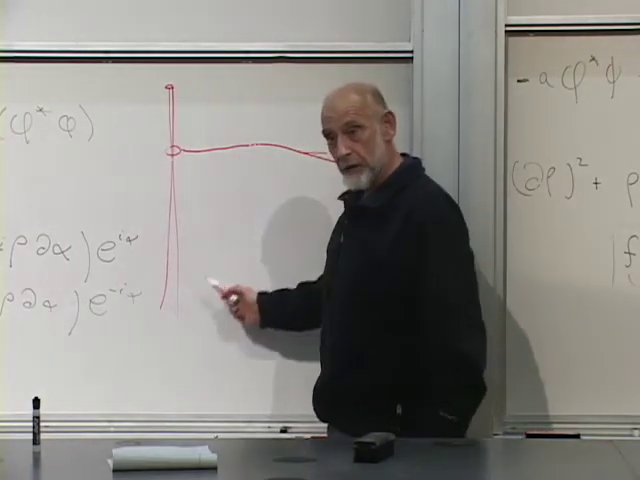
\includegraphics[width=0.68\textwidth]{lecture_07_figure_04.png}
\caption{골드스톤 모드의 비유를 위해 그린, 천천히 변하는 줄의 형상. 물리적으로 중요한 것은 장파장 변형의 작은 기울기이지 곡선의 수직 위치가 아니다.}
\lectureframe{01:04:19}
\end{figure}

\begin{classroomqa}
\audiencequestion{줄이 운동량은 0이면서 진동 에너지를 가질 수 있나요?
\lecturetimestamp{01:04:41}}
\lecturerresponse{수직 방향의 역학적 운동량과 줄을 따라 전달되는 파동의 운동량을 구별해야 한다. 정상파는 \(+k\)과 \(-k\)을 갖는 모드들의 중첩이어서 순운동량이 0일 수 있지만, 그래도 에너지를 전달한다. 장 이론의 비유에서 운동량은 축을 따라가는 파수를 뜻하고, 수직 변위는 내부 장 좌표를 나타낸다.}
\end{classroomqa}

슬링키는 종파의 비유를 제공한다. 이상화한 무한 슬링키를 축을 따라 통째로 옮겨도 아무것도 변하지 않는다. 이웃한 부분들을 조금씩 다른 거리만큼 옮기면 부드러운 압축파가 생긴다. 고체나 유체에서도 장파장 소리는 이와 비슷하게 집단 변위와 밀도 변화에서 비롯된다. 스핀파, 횡방향 줄파, 소리는 미시적으로 같은 들뜸은 아니지만 결정적인 양상은 공유한다. 균일한 연속 연산에는 에너지가 들지 않고, 그것이 천천히 변하는 형태로 나타나면 연성 모드가 된다.
\editorialnote{결정에서는 음향 포논을 자발적으로 깨진 연속 병진 대칭성의 난부--골드스톤 모드로 기술하는 것이 일반적이다. 줄과 슬링키는 같은 미분항만으로 이루어진 에너지 구조를 드러내기 위해 강의에서 사용한 역학적 비유다.}

이 용어는 짧은 강의실 농담을 할 만큼 중요하다. 이들은 제프리 골드스톤의 이름을 딴 \emph{골드스톤} 보손이지, 게이지 보손이 아니다. 강의에서는 골드스톤이 서스킨드의 친구였다고 언급한 뒤, 이와 실제로 다른 주제인 게이지 불변성으로 넘어간다.

\section{전역 위상 대칭성에서 게이지 대칭성으로}

\(U(1)\) 위상 대칭성은 전하 보존과 관련된 대칭성으로 이미 강의에서 다룬 바 있다. 하전 입자 장은 복소수이며, 이런 장에 공통 위상 인자를 곱해도 전역 이론은 변하지 않는다. 직관을 위해 전기적 전하라고 말할 수 있지만, 그 전하는 다른 \(U(1)\) 양자수일 수도 있다. 실제 광자는 질량이 없다. 궁극적으로 살펴볼 대상은 질량이 있는 \(Z\) 같은 광자형 장이다.

새로운 질문은 다음 변환이
\begin{equation}
  \phi'(x)=e^{i\theta(x)}\phi(x)
  \label{eq:l07-local-u1}
\end{equation}
\(\theta\)이 시공간에 걸쳐 임의로 변해도 대칭성이 될 수 있는가이다. 함수 \(\theta(x)\)는 변환 매개변수이지, 추가적인 동역학적 장이 아니다. 이 제안을 미분하여 확인해 보자.
\begin{equation}
  \partial_\mu\phi'
  =e^{i\theta}
   \left[\partial_\mu\phi+i(\partial_\mu\theta)\phi\right].
  \label{eq:l07-local-derivative}
\end{equation}
상수 \(\theta\)일 때는 추가 항이 없었다. 켤레장에 대해서는
\begin{equation}
  \partial_\mu\phi^{*\prime}
  =e^{-i\theta}
   \left[\partial_\mu\phi^*-i(\partial_\mu\theta)\phi^*\right].
\end{equation}
을 얻는다. 두 식의 곱은
\begin{align}
  \partial_\mu\phi^{*\prime}\partial^\mu\phi'
  ={}&
  \partial_\mu\phi^*\partial^\mu\phi
  i\left(
      \phi\,\partial_\mu\phi^*
      -\phi^*\partial_\mu\phi
    \right)\partial^\mu\theta
  \nonumber\\
  &+\phi^*\phi\,
    \partial_\mu\theta\,\partial^\mu\theta.
  \label{eq:l07-local-failure}
\end{align}
이다. \(\phi^*\phi\)는 불변이므로 퍼텐셜은 여전히 불변이지만, 보통의 운동항은 불변이 아니다. 전역 대칭성이 저절로 국소 대칭성이 되는 것은 아니다.

\begin{classroomqa}
\audiencequestion{멕시코 모자 그림에서 이런 실패는 원형 골짜기 주변에 굴곡이 있다는 뜻인가요?
\lecturetimestamp{01:19:37}}
\lecturerresponse{아닙니다. 퍼텐셜은 각도 방향으로 완벽히 평평할 수 있습니다. 위상이 시공간의 점마다 달라질 때 기울기 때문에 비용이 생기는 것입니다. 이는 골짜기가 울퉁불퉁해진다는 뜻이 아니라 보통의 미분항이 공간적 변화를 감지한다는 뜻입니다.}
\end{classroomqa}

\subsection{상쇄 역할을 하는 벡터장}

자연에 존재하는 광자, \(W\), \(Z\) 및 글루온의 상호작용은 강체 변환만이 아니라 국소 게이지 대칭성으로 구성된다. 국소 위상 변환을 대칭성으로 만들려면 사벡터 장 \(A_\mu\)을 이론에 추가해야 한다. 전자기학에서 \(A_0\)은 스칼라 퍼텐셜이며, 세 공간 성분은 벡터 퍼텐셜을 이룬다. 이들의 미분으로 전기장과 자기장을 구성한다.

내부적으로 일관된 다음 관례를 택하자.
\begin{equation}
  \phi'=e^{i\theta}\phi,
  \qquad
  A'_\mu=A_\mu-\partial_\mu\theta,
  \qquad
  D_\mu=\partial_\mu+iA_\mu.
  \label{eq:l07-gauge-convention}
\end{equation}
상쇄를 확인하는 과정에서 칠판의 부호 하나가 바뀌지만, 식 \eqref{eq:l07-gauge-convention}은 세 부호를 함께 정한다. 게이지 결합 상수와 전하는 일단 \(A_\mu\)에 흡수했다.
\editorialnote{\(q\)와 결합 상수 \(g\)를 명시하면 다음과 같이 쓸 수 있다.
\(D_\mu=\partial_\mu+igqA_\mu\) 및
\(A'_\mu=A_\mu-(gq)^{-1}\partial_\mu\theta\). 강의에서는 상쇄가 잘 드러나도록 이 상수들을 생략했다.}

켤레장에 대해서는
\begin{equation}
  D_\mu\phi^*=\partial_\mu\phi^*-iA_\mu\phi^*.
\end{equation}
을 얻는다. 이제
\begin{align}
  D'_\mu\phi'
  &=
  \left(\partial_\mu+iA'_\mu\right)e^{i\theta}\phi
  \nonumber\\
  &=
  e^{i\theta}
  \left[
    \partial_\mu\phi+i(\partial_\mu\theta)\phi
    +i(A_\mu-\partial_\mu\theta)\phi
  \right]
  \nonumber\\
  &=e^{i\theta}D_\mu\phi.
  \label{eq:l07-covariant-transform}
\end{align}
이다. \(\theta\)의 원치 않는 미분항은 \(A_\mu\)의 변환으로 상쇄된다. 마찬가지로
\begin{equation}
  D'_\mu\phi^{*\prime}=e^{-i\theta}D_\mu\phi^*.
\end{equation}
이고, 두 식의 곱은 불변이다. \emph{공변} 미분이라는 말은 미분한 양이 장 자체와 같은 간단한 방식으로 변환한다는 뜻이다.

\section{게이지 장의 동역학}

미분항을 고치기 위해 \(A_\mu\)만 도입하면 그 자체의 동역학이 없게 된다. 게이지 불변인 장세기는 다음과 같다.
\begin{equation}
  F_{\mu\nu}
  =\partial_\mu A_\nu-\partial_\nu A_\mu.
  \label{eq:l07-field-strength}
\end{equation}
장세기는 반대칭이므로 \(F_{\mu\mu}=0\)이다. 시간--공간 성분에는 전기장이 들어 있고, 공간--공간 성분에는 자기장이 들어 있다. 익숙한 3차원 벡터 표현에서 전자기장 에너지 밀도는 \(\bm E^2+\bm B^2\)에 비례하고, 로런츠 라그랑지안은 \(\bm E^2-\bm B^2\)에 비례한다. 부호는 계량 관례에 따라 달라진다.

\begin{classroomqa}
\audiencequestion{전자기장의 에너지와 라그랑지안은 무엇인가요?
\lecturetimestamp{01:33:20}}
\lecturerresponse{에너지는 \(E^2+B^2\)로 이루어지고, 라그랑지안에는 \(E^2-B^2\)이 쓰인다. 공변적으로는 후자를 \(F_{\mu\nu}F^{\mu\nu}\)의 관례적인 상수배로 쓴다. 반대칭 텐서는 벡터 퍼텐셜의 4차원 컬이다.}
\end{classroomqa}

장세기 자체는 게이지 불변이다.
\begin{align}
  F'_{\mu\nu}
  &=
  \partial_\mu(A_\nu-\partial_\nu\theta)
  -\partial_\nu(A_\mu-\partial_\mu\theta)
  \nonumber\\
  &=
  F_{\mu\nu}
  -\partial_\mu\partial_\nu\theta
  +\partial_\nu\partial_\mu\theta
  =F_{\mu\nu}.
  \label{eq:l07-field-strength-invariant}
\end{align}
마지막 등식은 보통의 혼합 편미분이 서로 교환된다는 사실에서 따른다. 따라서 표준적인 게이지 불변 라그랑지안은 다음과 같다.
\begin{equation}
  \boxed{
  \mathcal L
  =(D_\mu\phi)^*D^\mu\phi
  -V(\phi^*\phi)
  -\frac14F_{\mu\nu}F^{\mu\nu}}
  \label{eq:l07-scalar-qed}
\end{equation}
계량에 대해 선택한 부호와 정규화 관례는 별도로 두었다.

\begin{figure}[htbp]
\centering
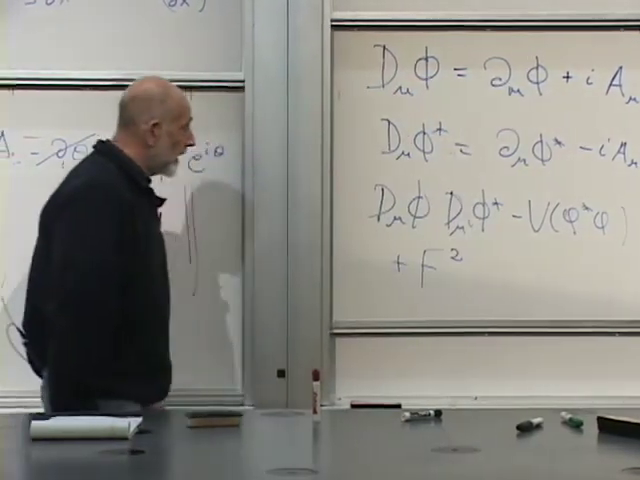
\includegraphics[width=0.84\textwidth]{lecture_07_figure_05.png}
\caption{칠판에 적힌 공변 미분과 조립된 게이지 불변 라그랑지안. 변환 구조가 잘 드러나도록 수치 계수는 생략했다.}
\lectureframe{01:38:45}
\end{figure}

이 구성은 전역 \(U(1)\) 대칭성을 국소 대칭성으로 확장하지만, 그 대가------로 새로운 벡터장을 도입한다. 아벨 예에서 그 장은 전자기 퍼텐셜이다.

\begin{classroomqa}
\audiencequestion{처음의 라그랑지안에는 보통의 미분이 쓰였습니다. 이를 공변 미분으로 바꾸고 그 결과를 실제 이론이라고 불러도 되는 이유가 무엇인가요?
\lecturetimestamp{01:42:55}}
\lecturerresponse{우리는 새로운 확장 이론, 즉 하전 물질과 게이지 장으로 이루어진 이론을 구성하는 중이다. 국소 게이지 불변성이 두 요소의 결합을 결정한다. 그렇게 얻은 양자 이론은 수학적으로 일관된 구조이며, 자연이 광자와 약한 게이지 장을 구성하는 방식과 일치한다. 상대론적 벡터 장을 일관성 없이 결합하면 비물리적 편극이나 확률 보존 위반이 생길 수 있다. 따라서 게이지 원리는 기존 자유 스칼라 이론을 겉으로만 바꿔 쓴 것이 아니다.}
\end{classroomqa}

\begin{classroomqa}
\audiencequestion{새로운 장을 더하는 것이 수정의 핵심적인 정당화 근거인가요?\lecturetimestamp{01:44:57}}
\lecturerresponse{그렇습니다. \(A_\mu\)가 없으면 국소적으로 회전한 장의 미분에 상쇄되지 않은 \(\partial_\mu\theta\)가 남습니다. \(A_\mu\)와 그 변환 법칙을 도입하면 이 항들이 상쇄됩니다. 기하학의 언어로는 \(A_\mu\)가 다발 위의 접속입니다. 이보다 깊은 수학은 실제로 유용하지만, 여기서는 위의 대수적 전개에 필요한 내용이 모두 담겨 있습니다.}
\end{classroomqa}

\section{게이지 보손에 질량항을 직접 넣을 수 없는 이유}

일반적인 보손 장의 질량은 이차항으로 나타냅니다. 다음 항을 더하고 싶을 수 있습니다.
\begin{equation}
  \Delta\mathcal L_{\rm Proca}
  =\frac12m^2A_\mu A^\mu.
  \label{eq:l07-proca}
\end{equation}
\(A_\mu\mapsto A_\mu-\partial_\mu\theta\) 아래에서,
\begin{equation}
  A'_\mu A^{\mu\prime}
  =
  A_\mu A^\mu
  -2A^\mu\partial_\mu\theta
  +\partial_\mu\theta\,\partial^\mu\theta,
\end{equation}
따라서 식~\eqref{eq:l07-proca}은 게이지 불변이 아닙니다. 국소 대칭성을 유지하면서 이 게이지 이론에 질량을 임의로 넣을 수는 없습니다.

\begin{figure}[htbp]
\centering
\includegraphics[width=0.72\textwidth]{lecture_07_figure_07.png}
\caption{제안된 벡터 보손의 질량항
\(\tfrac12m^2A_\mu A^\mu\)은 \(A_\mu\mapsto A_\mu-\partial_\mu\theta\) 아래에서 불변이 아닙니다. 이 실패가 힉스 메커니즘으로 이어지는 장애물입니다.}
\lectureframe{01:39:48}
\end{figure}

이것이 겉보기에 막다른 상황입니다. 게이지 불변성은 광자가 질량이 없는 이유를 설명하고, 비물리적 자유도가 이론에 들어오는 것을 막아 주지만, \(W\)와 \(Z\)는 질량이 있습니다. 이 난관을 벗어나기 위해 벡터 질량을 명시적으로 넣을 수는 없습니다. 게이지 불변 라그랑지안에 이미 들어 있는 장들에서 해법이 나와야 합니다.

\begin{classroomqa}
\audiencequestion{게이지 불변성을 도입하는 것 자체가 골드스톤 보손을 만들어 내나요?\lecturetimestamp{01:45:51}}
\lecturerresponse{아닙니다. 골드스톤 보손은 벡터 퍼텐셜을 도입하기 전에 연속적인 \emph{전역} 대칭성이 자발적으로 깨지면서 생겼습니다. 대칭성이 국소 대칭성이 되면, 위상이 위치에 따라 변하더라도 \(A_\mu\)를 통해 그 변화를 상쇄할 수 있습니다. 대칭성이 깨진 게이지 이론에서는 각도 모드가 더 이상 독립적인 질량 없는 입자가 아닙니다. 그 모드는 이제 질량을 갖게 된 벡터 장의 추가 편극을 제공합니다. 다음 강의에서는 이 내용을 단순히 선언하는 데 그치지 않고 유도하겠습니다.}
\end{classroomqa}

\begin{classroomqa}
\audiencequestion{이 내용은 강이 굽이쳐 흐르는 이유도 설명하나요?\lecturetimestamp{01:47:03}}
\lecturerresponse{여기서는 직접적인 연관성이 알려져 있지 않습니다. 유체의 소용돌이와 생물의 형태도 대칭성 방법으로 기술할 수는 있습니다. 장론의 발상이 뜻밖의 곳에서 발견되더라도 놀랄 일은 아니지만, 이 강의는 강의 굽이침을 설명하는 게이지 이론을 제시하지 않습니다.}
\end{classroomqa}

\section{강의의 마무리}

이제 처음에 약속한 두 가지 요소를 갖추었습니다. 진공 상태들이 원을 이루는 연속적인 전역 대칭성에는 평평한 각도 방향이 있고, 그 방향의 느린 변화는 질량 없는 골드스톤 장이 됩니다. 국소 대칭성에는 게이지 접속과 공변미분이 필요하며, 식~\eqref{eq:l07-proca}에 나타난 직접적인 벡터 질량항은 허용되지 않습니다.

다음 단계에서는 식~\eqref{eq:l07-mexican-hat}의 대칭성이 깨진 퍼텐셜을 식~\eqref{eq:l07-scalar-qed}의 게이지 불변 이론에 넣겠습니다. 그러면 두 가지 일이 함께 일어납니다. 골드스톤 입자는 물리적 스펙트럼에서 사라지고, 벡터 장은 질량을 얻습니다. 통상적인 교육용 표현으로는 게이지 대칭성이 자발적으로 깨진다고 합니다. 더 정확히 말하면 게이지 중복성은 그대로 유지되고, 이론은 질량을 가진 벡터 들뜸이 존재하는 힉스 상에 놓입니다.
\editorialnote{국소 게이지 대칭성은 서로 다른 관측 가능한 상태 사이에서 작용하는 일반적인 물리적 대칭성이 아니라 기술상의 중복성입니다. 이 강의에서는 게이지 대칭성의 자발적 깨짐이라는 표준적인 약칭을 사용합니다. 게이지 불변인 물리적 진술은 힉스 상에서 자유도의 배열이 재편된다는 것입니다.}

이것이 힉스 현상입니다. 아직 이 현상을 직접 살펴보지는 않았습니다. 이번 강의에서는 문제를 충분히 정확하게 정식화하는, 꼭 필요하지만 더 어려운 작업을 했습니다. 그래서 해법이 제시되면 피할 수 없는 결론이 될 것입니다.